\subsection{Extraction of prompt and nonprompt \texorpdfstring{\JPsi}{J/psi} mesons}\label{sec:Charmonia_Analysis_JPsiYieldExtraction}

This section describes the procedure used to extract the yields of prompt and nonprompt \JPsiToMuMu candidates in \Runpp and \RunPbPb collision data. Considering the large lifetime of b hadrons ($\tau_{\B} \sim \SI{1.5}{\ps}$), the prompt and nonprompt \JPsi mesons are distinguished by virtue of the pseudoproper-decay length \ctau, determined from the displacement between the primary collision and secondary \mumu vertices, as detailed in \sect{sec:Charmonia_Analysis_JPsiYieldExtraction_CtauDef}.

The \JPsi-meson yields are extracted by performing a two-dimensional unbinned-maximum likelihood fit to the \mumu invariant mass (\mMuMu) and \ctau distributions (hereafter referred as 2D fit), performed with the RooFit framework~\cite{RooFit}. The expression of the total functional form $F(\mMuMu,\ctau)$, used in the 2D fit, is defined as:

\begin{equation}
 F\left(\mMuMu,\ctau\right) = \sum\limits_{i=\JPsi,\bkg}N_{i} \cdot M_{i}\left(\mMuMu\right) \cdot D_{i}\left(\ctau\right) \otimes R_{i}\left(\ctau\right)
 \label{eq:2DFit}
\end{equation}

where $\otimes$ represents a convolution with respect to the \ctau variable, \nJPsi is the number of inclusive \JPsi mesons (i.e. including prompt and nonprompt \JPsi mesons), \nbkg is the number of background dimuons, $R_{\JPsi}$ ($R_{\bkg}$) represents the \ctau resolution of signal (background) dimuons, and $M_{i}$ and $D_{i}$ are the \mMuMu and \ctau functional forms for each event source, respectively.

The 2D fits are done in four rapidity intervals corresponding to 0-0.6, 0.6-1.2, 1.2-1.8 and 1.8-2.4. In the most forward rapidity region ($1.8 < |\rapMuMu| < 2.4$), the \JPsi-meson yields are extracted down to 3~\GeVc, while in the other rapidity regions ($|\rapMuMu| < 1.8$) they are extracted down to 6.5~\GeVc, reflecting the CMS detector acceptance. The signal extraction is also performed in several centrality bins with the following boundaries: [0, 5, 10, 15, 20, 25, 30, 35, 40, 45, 50, 60, 70, 100\%] at $|\rapMuMu| < 2.4$ and [0, 10, 20, 30, 40, 50, 100\%] in each of the rapidity intervals. The full set of analysis bins used in the \JPsi-meson analysis is listed in \app{app:Charmonia_Binning}.

Due to the complexity of the 2D functional form and the limited statistics to fully constrain all its parameters at the same time, the 2D fits are performed in four sequential steps:
\begin{enumerate}
 \item The \mMuMu shape of the signal is parametrised using a weighed sum of two Crystal Ball functions, while the background is described with a Chebyshev function (\sect{sec:Charmonia_Analysis_JPsiYieldExtraction_InvMassPar}). The \mMuMu functional form is fitted on data and the corresponding parameters are fixed in this step.
 \item The shape of the \ctau resolution is determined from data by fitting the $\ctau < 0$ distribution with a weighed sum of three Gaussian distributions, taking into account the \ctau uncertainty in each event (\sect{sec:Charmonia_Analysis_JPsiYieldExtraction_CtauResPar}).
 \item The \ctau true lineshape of the nonprompt \JPsi mesons is parametrised with an exponential function, while the nonprompt component of the background is parametrised with a weighed sum of three exponential functions (\sect{sec:Charmonia_Analysis_JPsiYieldExtraction_CtauPar}). The \ctau functional form, derived by convolving the \ctau true lineshape with the \ctau resolution model, is fitted on data and the parameters of the \ctau true lineshapes are constrained in this step.
 \item The \ctau and \mMuMu distributions in data are fitted with the 2D functional form $F(\mMuMu,\ctau)$ (\sect{sec:2Dfits}), and the prompt and nonprompt \JPsi meson yields are extracted (\sect{sec:JPsiYields}).
\end{enumerate}

A detailed description of each step is provided in Sections \ref{sec:Charmonia_Analysis_JPsiYieldExtraction_InvMassPar} to \ref{sec:2Dfits}. An example of the 2D fit results projected along the \mMuMu and \ctau variables are shown in \fig{fig:2DFits_proj}, extracted from \RunPbPb collision data.

\begin{figure}[htb!]
 \centering
 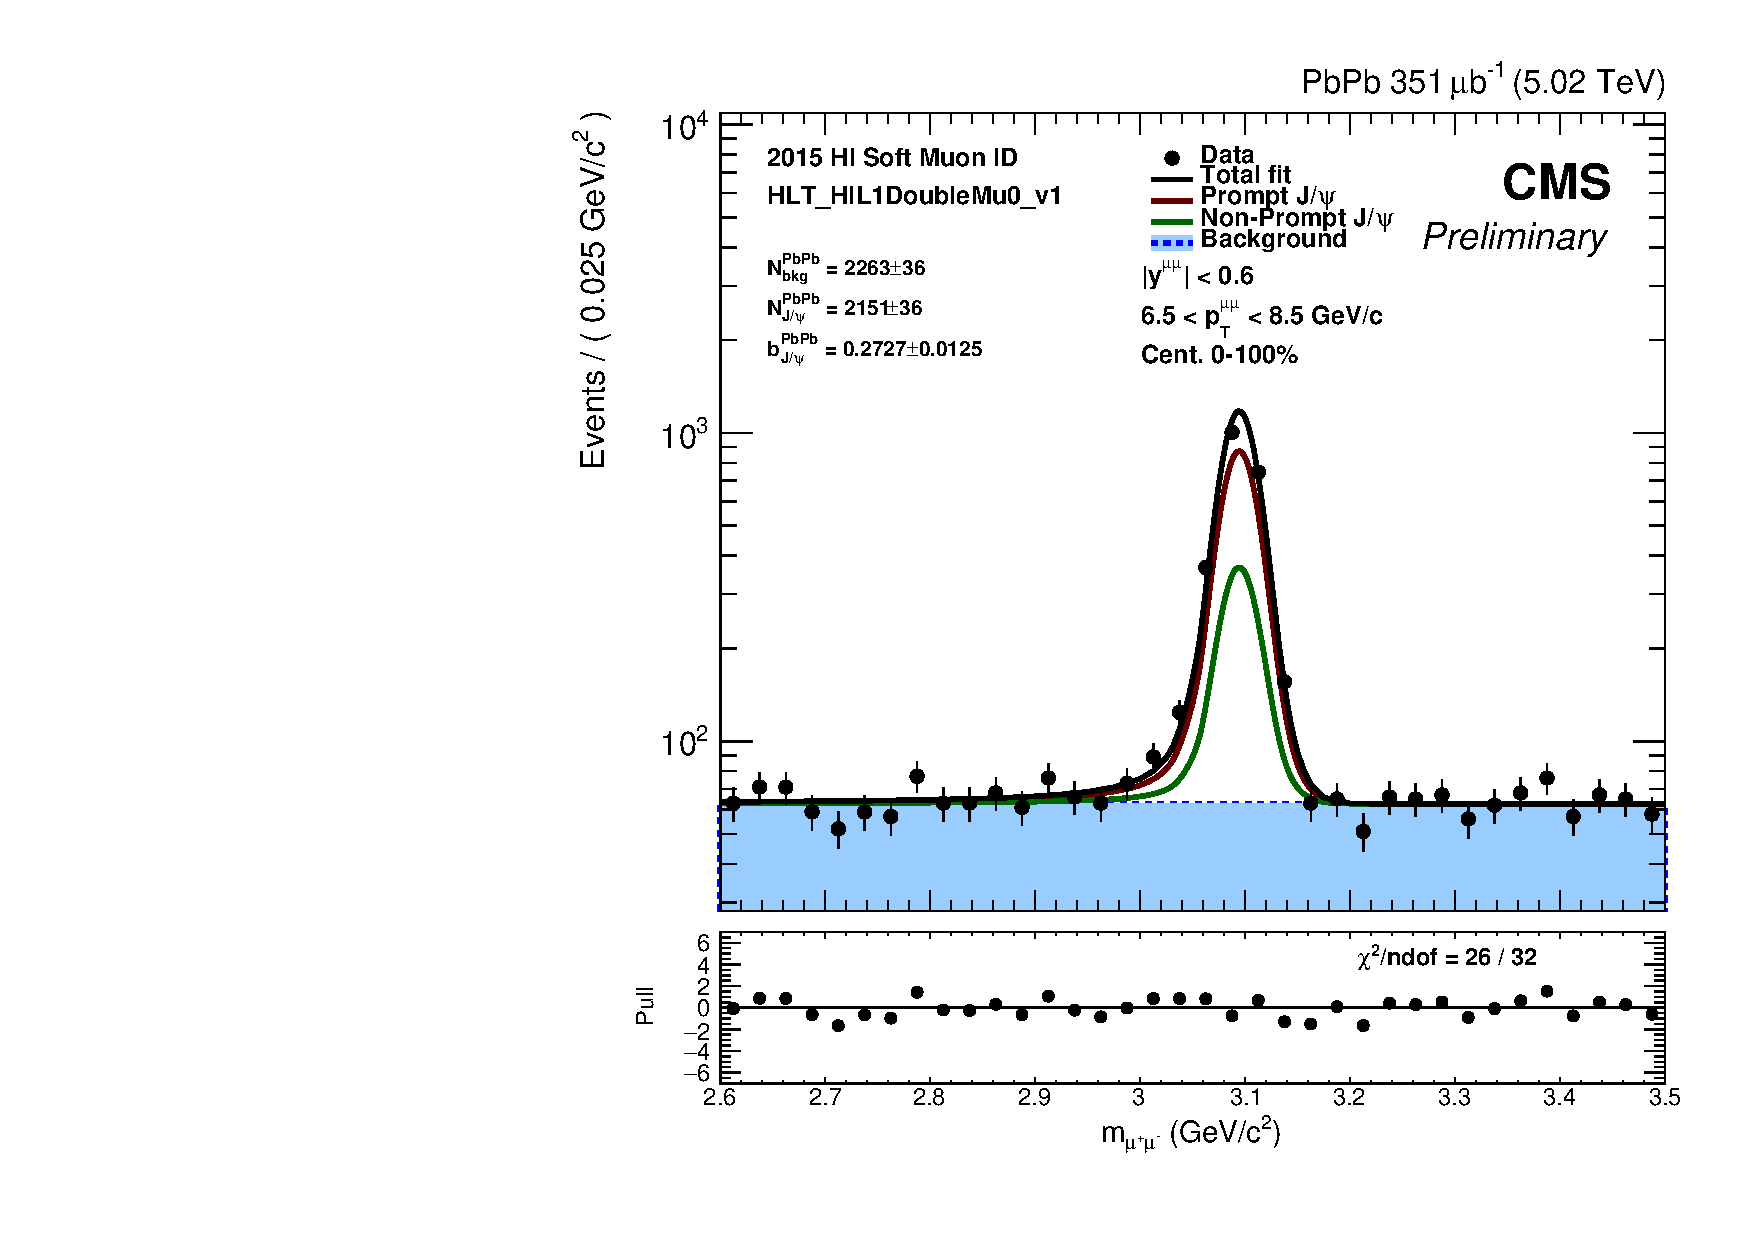
\includegraphics[width=0.45\textwidth]{Figures/Charmonia/Analysis/JpsiSignalExtraction/2Dfits/PLOT_MASS_DATA_PbPb_Bkg_Uniform_BkgNoPR_TripleDecay_CtauRes_TripleGaussianResolution_Jpsi_DoubleCrystalBall_JpsiNoPR_SingleSidedDecay_pt6585_rap06_cent0200.pdf}
 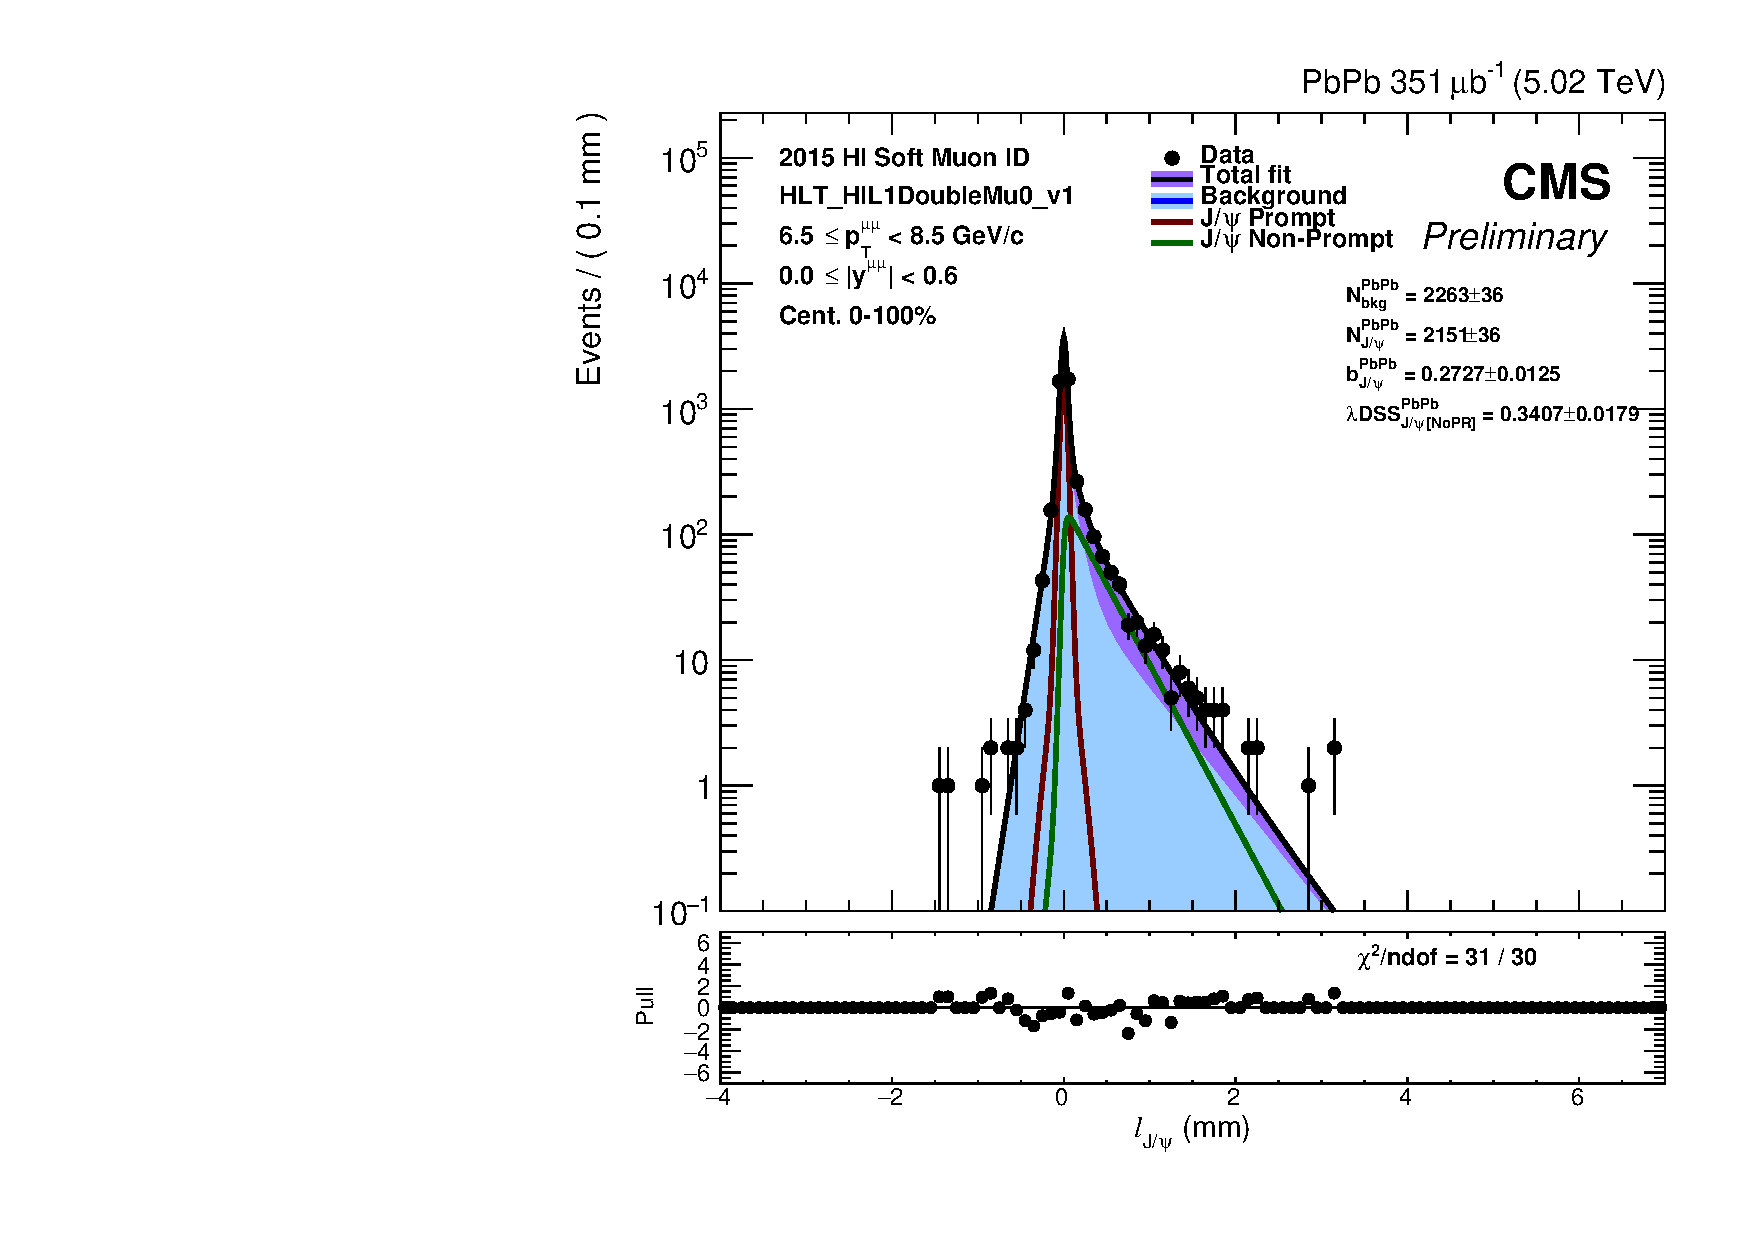
\includegraphics[width=0.45\textwidth]{Figures/Charmonia/Analysis/JpsiSignalExtraction/2Dfits/PLOT_CTAU_DATA_PbPb_Bkg_Uniform_BkgNoPR_TripleDecay_CtauRes_TripleGaussianResolution_Jpsi_DoubleCrystalBall_JpsiNoPR_SingleSidedDecay_pt6585_rap06_cent0200.pdf}
 \caption{Results of the 2D fits performed on \RunPbPb data, projected onto the dimuon invariant mass (left) and pseudoproper-decay length (right) variables.} 
 \label{fig:2DFits_proj}
\end{figure}


\subsubsection{Definition of pseudoproper-decay length}\label{sec:Charmonia_Analysis_JPsiYieldExtraction_CtauDef}

The pseudoproper-decay length \ctau of \mumu candidates, used to estimate the b-hadron decay length, is defined as:

\begin{equation}
 \ctau = \mJPsi\cdot\frac{\pMuMuvec \cdot \vec{r}}{\left(\pMuMu\right)^{2}}
\end{equation}

where $\mJPsi = 3.0969~\GeVcc$ is the mass of the \JPsi meson~\cite{PDG}, $\pMuMuvec$ is the dimuon momentum vector and $\vec{r}$ is the displacement vector between the position of the primary collision vertex and the dimuon vertex.

The primary collision vertex is reconstructed by fitting the position, along the beam axis, of all tracks produced promptly within a radius of \SI{5}{\cm} from the interaction region, while the secondary \mumu vertex is determined by extrapolating the position of closest approach between the two muon tracks. The vertex fit is performed using an adaptive vertex fitting algorithm~\cite{VertexFitter,VertexFitter_2}, which determines the best estimate of the vertex parameters, including its position and covariance matrix~\cite{CMSTracking}.

The uncertainty associated to the \ctau measurement, referred as \sigmactau, is computed as:

\begin{equation}
 \sigmactau = \sqrt{ \mJPsi \cdot \frac{\pMuMuvec \cdot S \cdot \pMuMuvec}{\left(\pMuMu\right)^{2}} } 
\end{equation}

where $S$ is the the sum of the covariance matrices associated to the primary collision and \mumu vertex fits. The pseudoproper-decay length is measured in the CMS detector with a resolution of \SI{35}{\um}, allowing to resolve the decay vertex of b hadrons.

\subsubsection{Dimuon invariant mass parametrisation}\label{sec:Charmonia_Analysis_JPsiYieldExtraction_InvMassPar}

The inclusive \JPsi meson and background yields are extracted by fitting the \mMuMu distribution in the dimuon invariant mass region $2.6< \mMuMu < 3.5~\GeVcc$. The main source of background in this mass region derives from pairs of uncorrelated muons produced from leptonic decays of kaons and pions, and semi-leptonic decays of heavy-flavour hadrons. These uncorrelated muon pairs are combined forming a continuous \mMuMu distribution (i.e. combinatorial background). On the contrary, the \JPsi mesons decay to correlated muon pairs producing a narrow peak (i.e. resonance) in the \mMuMu spectrum around $\mMuMu \approx 3.09~\GeVcc$. As a consequence, different functional forms are used to model the signal and background \mMuMu shapes.

\paragraph{Parametrisation of the \texorpdfstring{\JPsi}{J/psi}-meson invariant mass shape.} The \mMuMu distribution of inclusive \JPsi mesons is modelled with a weighed sum of two Crystal Ball (CB) functions. The Crystal Ball function consists of a Gaussian core and a power-law tail. The Gaussian core is parametrised with a width $\sigma_{\CB}$ and a mean \mJPsi, while the power-law tail is parametrised by an exponent \nnJPsi that accounts for energy loss due to final-state photon radiation and a parameter \aJPsi that determines the transition point between the Gaussian and the power-law functions, as defined in:

\begin{linenomath}
  \begin{align}
    \label{eq:CristalBall}
    \CB\left( m \right) = \left\{
      \begin{array}{ll}
        \frac{1}{\sqrt{2\pi}\,\sigma_{\CB}}\exp{ \left[ -\frac{1}{2} \left(\frac{m - \mJPsi}{\sigma_{\CB}}\right)^{2} \right] },& \text{if}~\left(\frac{m - \mJPsi}{\sigma_{\CB}}\right) > -\aJPsi\\[0.5cm]
        \frac{1}{\sqrt{2\pi}\,\sigma_{\CB}}\exp{ \left[ -\frac{\abs{\aJPsi}^2}{2} \right] }\left(\frac{\nnJPsi}{\abs{\aJPsi}}\right)^{\nnJPsi}\left( \frac{\nnJPsi}{\abs{\aJPsi}}-\abs{\aJPsi}- \frac{m - \mJPsi}{\sigma_{\CB}} \right)^{-\nnJPsi},& \text{if}~\left(\frac{m - \mJPsi}{\sigma_{\CB}}\right) \leq -\aJPsi
      \end{array}\right.
  \end{align}
\end{linenomath}

The total \mMuMu functional form of the signal is then given by:

\begin{equation}
 M_{\JPsi}\left(\mMuMu\right) = \fJPsi \cdot \CB_{1}\left(\mMuMu\right) + ( 1 - \fJPsi) \cdot \CB_{2}\left(\mMuMu\right)
\end{equation}

where the two Crystal Ball functions are defined with common mean \mJPsi and tail parameters \aJPsi and \nnJPsi, and  the two CB widths are constrained such that $\sigma_{\CB,2} \geq \sigma_{\CB,1}$.

The Crystal Ball parameters are optimised by fitting the prompt \JPsi-meson simulations. On the one hand, the parameters are found to be consistent within different collision systems and also as a function of collision centrality and dimuon \pt. On the other hand, the fits performed in the inclusive dimuon rapidity region ($\abs{\rapMuMu} < 2.4$) are different from those done in differential \rapMuMu regions. As a result, different sets of parameters are used for the differential and integrated rapidity regions,  extracted from the \Runpp and \RunPbPb prompt \JPsi-meson simulations. The set of parameters for the differential rapidity regions are determined from the corresponding rapidity-averaged values.

When fitting the \mMuMu distribution in \Runpp and \RunPbPb collision data, the tail parameters \aJPsi and \nnJPsi are fixed to the values extracted from simulation, while the ratio of CB widths ($\sigma_{\CB,2}/\sigma_{\CB,1}$) is also fixed to simulation only when fitting the \RunPbPb data. This is done because the data samples do not provide sufficient constraining power to reliably estimate the CB tail parameters. The set of parameters left free in both \Runpp and \RunPbPb data fits are \fJPsi, \mJPsi and $\sigma_{\CB,1}$, while $\sigma_{\CB,2}$ is left free only in the \Runpp data fits. The signal shape parameters extracted from simulations are summarised in \tab{tab:Avg_MCSignalShapeParam_rap}.

\begin{table}[htb!]
  \centering
  \smallskip
  \begin{tabular}{lcccc}
    \hline\hline
    Rapidity region & \fJPsi & \aJPsi & \nnJPsi & ${\sigma_{\CB,2}/\sigma_{\CB,1}}$ \\
    \hline
    Differential & 0.78 & \color{blue}{\textbf{2.10}} & \color{blue}{\textbf{1.35}}  & \color{red}{\textbf{1.68}}  \\
    $\abs{\rap} < 2.4$ & 0.58 & \color{blue}{\textbf{1.94}} & \color{blue}{\textbf{1.64}}  & \color{red}{\textbf{2.06}}
  \end{tabular}
  \caption{Parameters extracted from the prompt \JPsi-meson simulation and used to constrain the double Crystal Ball functions in each differential and integrated rapidity region. The parameters fixed to simulation in both \RunPbPb and \Runpp data fits are shown in bold blue colour, while those fixed to simulation only on \RunPbPb data are displayed in bold red colour. The \fJPsi values from simulation are only used to initialise them in the data fits.}
  \label{tab:Avg_MCSignalShapeParam_rap}
\end{table}

\paragraph{Parametrisation of the background invariant mass shape.} The \mMuMu distribution of background dimuons is described with a Chebyshev function of order $N$, defined as:

\begin{equation}
 M_{\bkg}^{N}\left(\mMuMu\right) = \sum_{i=0}^{N} {c_{i} T_{i}\left(\mMuMu\right)}
\end{equation}

where $T_{i}$ is a Chebyshev polynomial of order $i$ and $c_{i}$ is the corresponding fit parameter. The Chebyshev polynomials are determined using the following recurrence relation~\cite{ChebyshevPoli}:
\begin{equation}
  T_{0}\left(m\right) = 1 \quad\quad ; \quad\quad  T_{1}\left(m\right) = m \quad\quad ; \quad\quad  T_{i+1}\left(m\right) = 2mT_{i}\left(m\right) - T_{i-1}\left(m\right)
\end{equation}

The main advantage of using a Chebyshev function is that the fit parameters $c_{i}$ are fully uncorrelated between them, improving the convergence of the dimuon invariant mass fits. The order of the background \mMuMu model is varied between 0 and 6, and the best order for each analysis bin is chosen by performing a Log-Likelihood Ratio (LLR) test. The LLR test compares the resulting minimised Negative Log-Likelihood (NLL) of a Chebyshev fit of order $N$ to the NLL of a Chebyshev fit of order $N+1$ and $N+2$ (two subsequent orders are needed to account for the change between odd and even polynomials).

The difference between the NLL values derived from the fits using a Chebyshev polynomial of order $N$ and $M > N$, is proportional to a $\chi^2$ distribution with $2(M-N)$ number of degrees of freedom, in particular:

\begin{equation}
  \chi^{2}_{N \rightarrow N+1} = 2\cdot(\text{NLL}_{N} - \text{NLL}_{N+1}) \quad ; \quad
  \chi^{2}_{N \rightarrow N+2} = 2\cdot(\text{NLL}_{N} - \text{NLL}_{N+2})
 \label{eq:llr-test}
\end{equation}

For a given Chebyshev function of order $N$, the next order is considered to fit the data significantly better if the $\chi^{2}$ probabilities associated to the $N+1$ or $N+2$ orders are less than $5\%$. Thus, if in a given analysis bin, the next order does not significantly improve the quality of the fit, then the current order of the Chebyshev function is chosen. As an example, \tab{tab:LLRTEST} summarise the results of the LLR test performed in \RunPbPb data for dimuons within $0.6 < \abs{\rapMuMu} < 1.2$ and $9.5 \leq \ptMuMu < 11~\GeVc$, which in this case the first order is chosen since $p(\chi^{2}_{1 \rightarrow 2}, 2)$ and $p(\chi^{2}_{1 \rightarrow 3}, 4)$) are larger than $5\%$.

\begin{table}[htb!]
 \centering
 \begin{tabular}{ c c c c c c c }
  M & NLL & p(N = 0) & p(N = 1) & p(N = 2) & p(N = 3) & p(N = 4) \\
  \hline
  0 & -28534.76 &  &  &  &  & \\
  1 & -28537.94 & 4.2$\%$ &  &  &  & \\
  2 & -28538.08 & 15.6$\%$ & \textbf{86.8$\%$} &  &  & \\
  3 & -28538.44 & 28.9$\%$ & \textbf{90.9$\%$} & 69.8$\%$ &  & \\
  4 & -28538.82 & 42.3$\%$ & 94.1$\%$ & 83.3$\%$ & 68.8$\%$ & \\
  5 & -28538.93 & 59.7$\%$ & 98.2$\%$ & 94.6$\%$ & 91.4$\%$ & 89.4$\%$\\
  6 & -28539.40 & 67.9$\%$ & 98.3$\%$ & 95.5$\%$ & 92.7$\%$ & 88.2$\%$\\
 \end{tabular}
 \caption{Results of the LLR test used to determine the order of the Chebyshev function for the background  \mumu invariant mass fitted in \RunPbPb data within $0.6 < \abs{\rapMuMu} < 1.2$ and $9.5 \leq \ptMuMu < 11~\GeVc$. The LLR test results of which the $\chi^{2}$ probability determined for two consecutive orders ($M = N+1$ and $M = N+2$) are higher than $5\%$ are highlighted in bold.}
 \label{tab:LLRTEST}
\end{table}

Another example is given in \fig{fig:Mass}, where the fits to the dimuon invariant mass distribution in \RunPbPb and \Runpp collision data have been performed using a first order and second order Chebyshev function, respectively. Among all the analysis bins, the orders of the Chebyshev function selected by the LLR tests are no larger than first order in \RunPbPb fits and third order in \Runpp fits.

\begin{figure}[htb!]
 \centering
 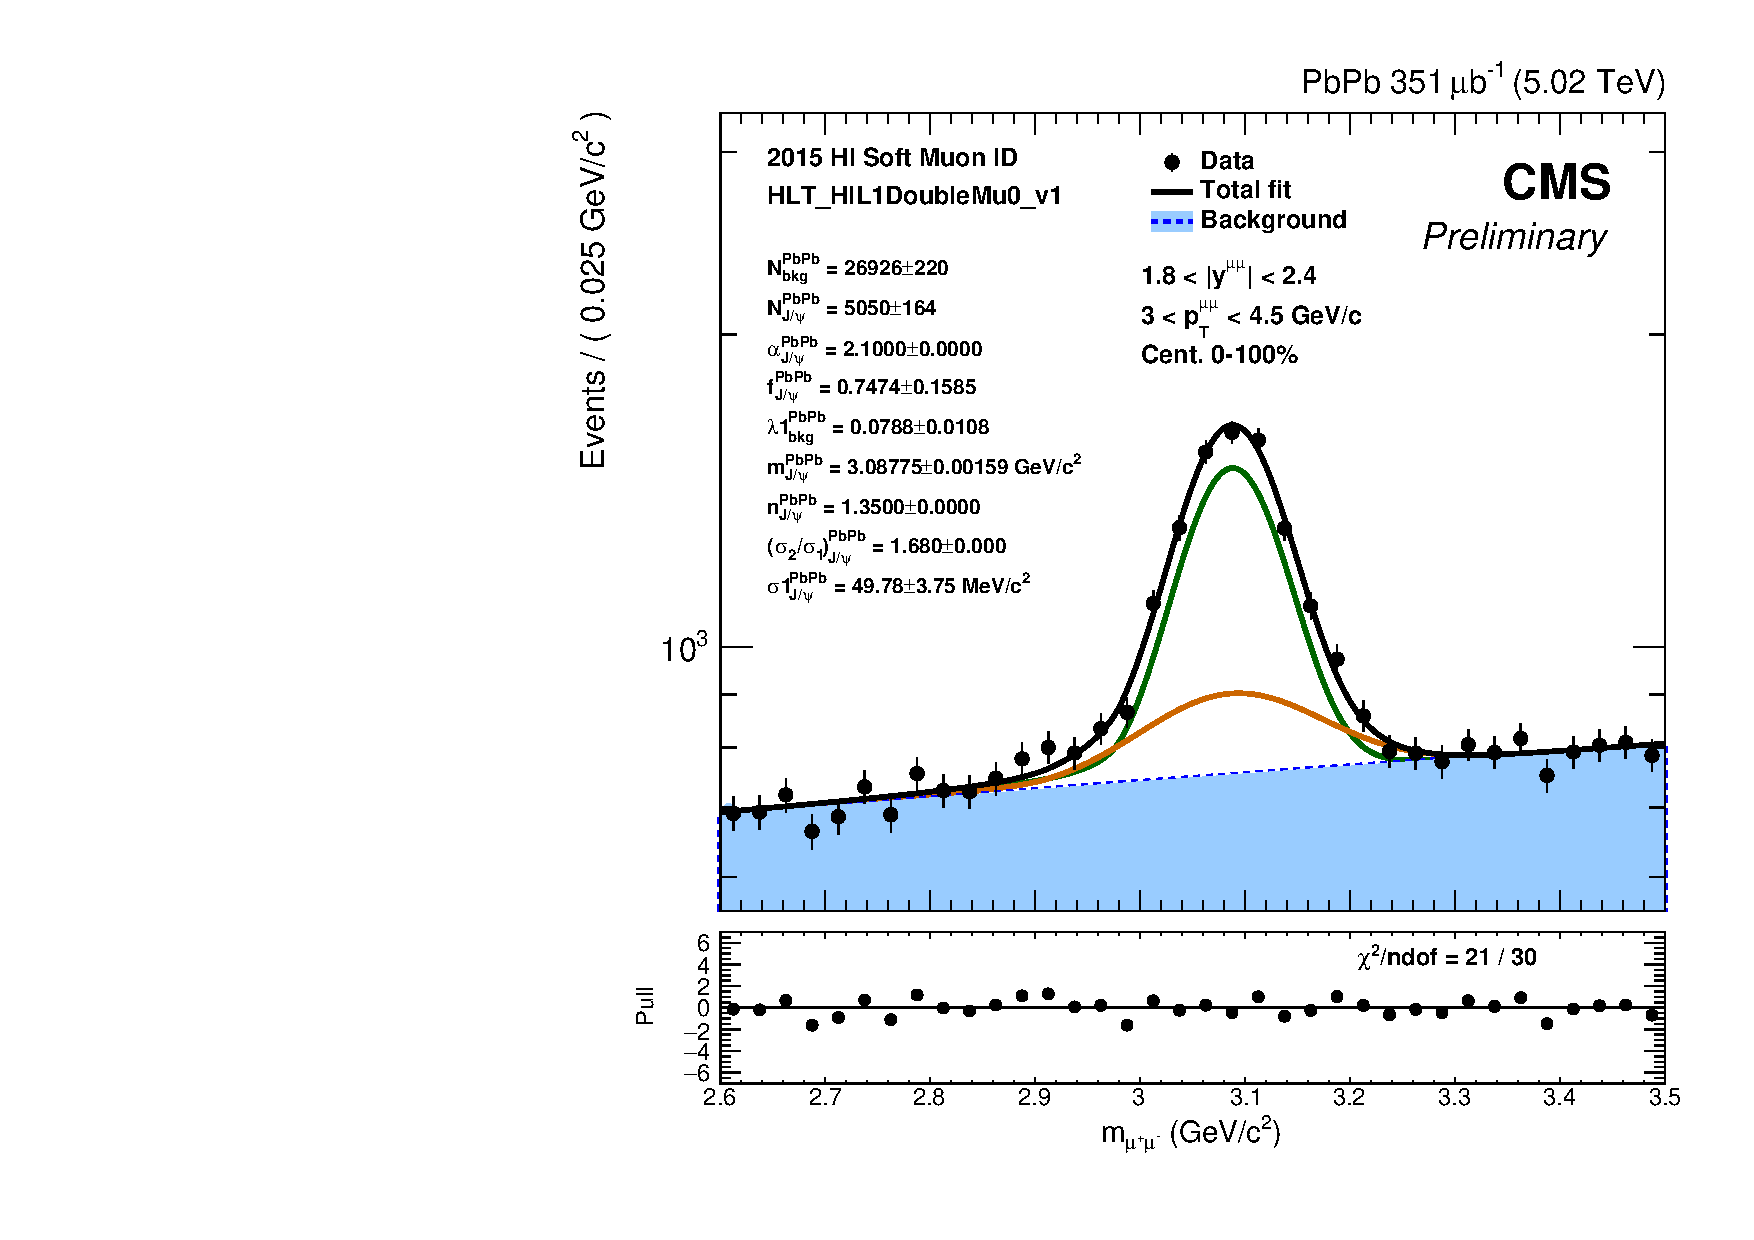
\includegraphics[width=0.45\textwidth]{Figures/Charmonia/Analysis/JpsiSignalExtraction/mass/PLOT_MASS_DATA_PbPb_Jpsi_DoubleCrystalBall_pt3045_rap1824_cent0200.pdf}
 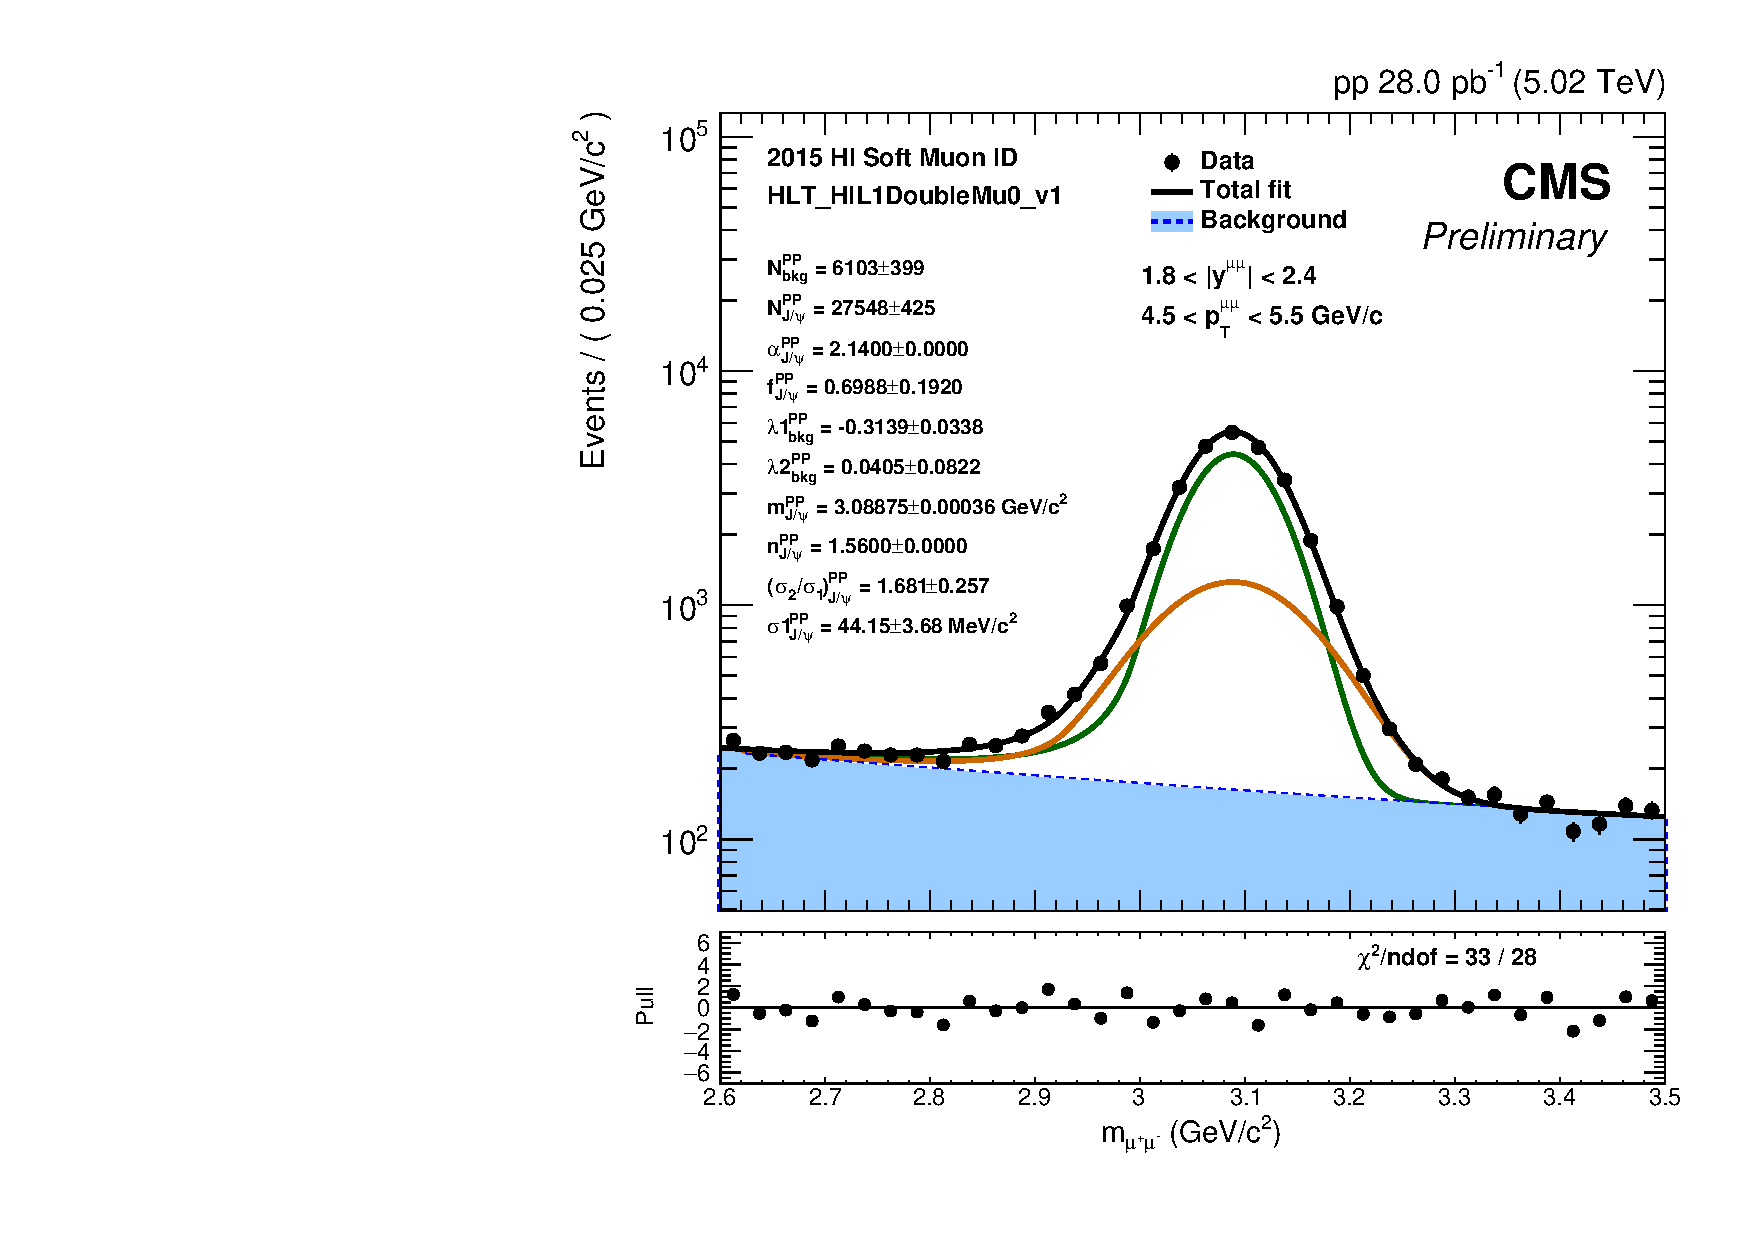
\includegraphics[width=0.45\textwidth]{Figures/Charmonia/Analysis/JpsiSignalExtraction/mass/PLOT_MASS_DATA_PP_Jpsi_DoubleCrystalBall_Bkg_Chebychev2_pt4555_rap1824_cent0200.pdf}
\caption{Results of the fits to the \mumu invariant mass distribution in \RunPbPb (left) and \Runpp (right) data. The black line represents the total fit model while the blue filled area represents the fitted background shape.}
 \label{fig:Mass}
\end{figure}

\subsubsection{Pseudoproper-decay length resolution}\label{sec:Charmonia_Analysis_JPsiYieldExtraction_CtauResPar}

The \ctau resolution depends on the measurement of the dimuon momentum and its vertex position, and as a result, it is affected by the \ctau uncertainty (\sigmactau) of each event. In addition, since the \sigmactau depends on the \pt and rapidity of dimuon candidates, the \sigmactau distribution may differ between background and signal dimuons. In order to take into account the \ctau uncertainty in each event, the \ctau resolution of signal and background dimuons is modelled with:

\begin{equation}
 R_{\JPsi(\bkg)}\left(\ctau\right) = \int{\dd{\sigmactau}} R\left(\ctau | \sigmactau\right) \cdot \Punzi_{\JPsi(\bkg)}\left(\sigmactau\right)
 \label{eq:CtauFit}
\end{equation}

where $R(\ctau | \sigmactau)$ is the functional form of the \ctau resolution depending on \sigmactau, and $\Punzi_{\JPsi(\bkg)}(\sigmactau)$ represents the signal (background) \sigmactau distribution.

Using this approach, the \ctau resolution is adjusted for each event to the measured \ctau uncertainty weighed by the corresponding \sigmactau distribution for signal and background dimuons. The parametrisation of the \ctau resolution and the determination of the \sigmactau distributions are detailed as follows.

\paragraph{Extraction of the \sigmactau distribution.} The distribution of \sigmactau is described using a template histogram determined from data. The corresponding \sigmactau distributions for signal and background dimuons are extracted using the statistical technique called \sPlot~\cite{sPlot}.

The \sPlot technique can be applied to a multivariate data sample made of a combination of several sources of events (e.g. signal and background), where each event is described by a set of variables divided in two categories. The first category consists of discriminating variables whose distributions are known for each source of events, while the second category corresponds to a set of variables, called control variables, whose distributions for some sources are unknown. The \sPlot technique allows to reconstruct the distribution of the control variables for each source, by weighing the events with the so-called $_{s}{Weights}$, computed with the information of the discriminating variables.

In the \JPsi meson analysis, the \mumu invariant mass is used as discriminating variable in order to determine the signal and background distributions of \sigmactau. The corresponding \sWeights are derived  using the \mMuMu functional forms of each source ($M_{\JPsi}$ and $M_{\bkg}$), obtained in \sect{sec:Charmonia_Analysis_JPsiYieldExtraction_InvMassPar}, in the following way:

\begin{equation}
 \begin{split}
  \sW_{i}\left(\mMuMu\right) &= \frac{\sum_{j = \left\{\JPsi, \bkg\right\}}{ V_{i, j} \cdot M_{j}\left(\mMuMu\right) } }{ \sum_{j = \left\{\JPsi, \bkg\right\}}{ N_{j} \cdot M_{j}\left(\mMuMu\right) } } \quad , \quad \text{for} \quad i = \JPsi , \bkg
 \end{split}
\end{equation}

where $N_{j}$ is the number of dimuon events from source $j$, and $V_{i, j}$ is the element of the covariance matrix associated to the $i^{\text{th}}$ and $j^{\text{th}}$ source ($i, j =$ \JPsi and background). The covariance matrix of each source is computed by inverting the following matrix:

\begin{equation}
 V^{-1}_{i, j} = \frac{ M_{i}\left(m_{\mu \mu}\right) \cdot M_{j}\left(m_{\mu \mu}\right) }{  \sum_{i = \left\{\JPsi, bkg\right\}}{ N_{i} \cdot M_{i}\left(m_{\mu \mu}\right) } }
\end{equation}

Once determined, the $\sW_{\JPsi}$ and  $\sW_{\bkg}$ weights are then applied to each event to create a signal-like and a background-like dataset. Each dataset is subsequently projected onto the \sigmactau variable, to extract the signal and background \sigmactau distributions and form \sigmactau template histograms for each source. An example of a \sigmactau distribution in \Runpp and \RunPbPb collision data is presented in \fig{fig:errDistr}.

\begin{figure}[htb!]
 \centering
 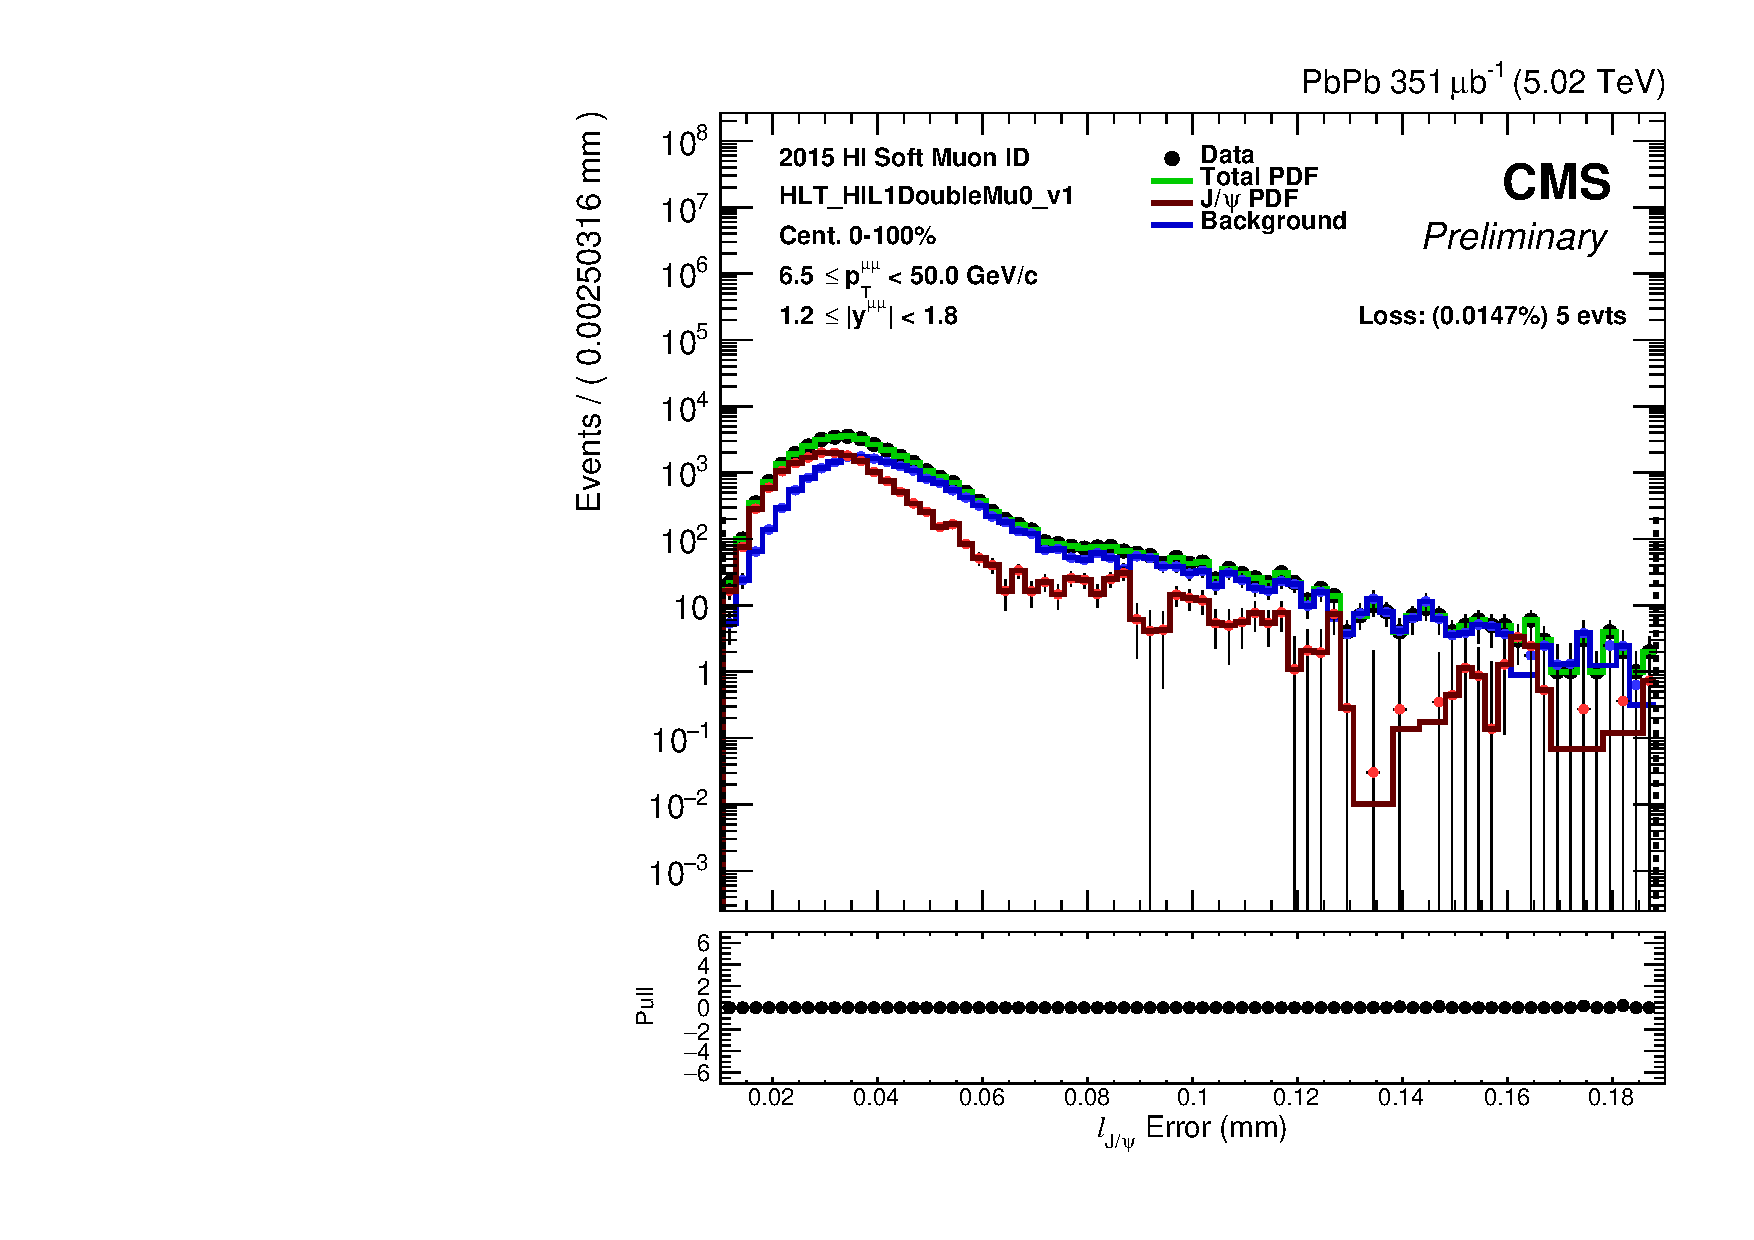
\includegraphics[width=0.45\textwidth]{Figures/Charmonia/Analysis/JpsiSignalExtraction/ctauError/PLOT_CTAUERR_DATA_PbPb_Jpsi_Bkg_pt65500_rap1218_cent0200.pdf}
 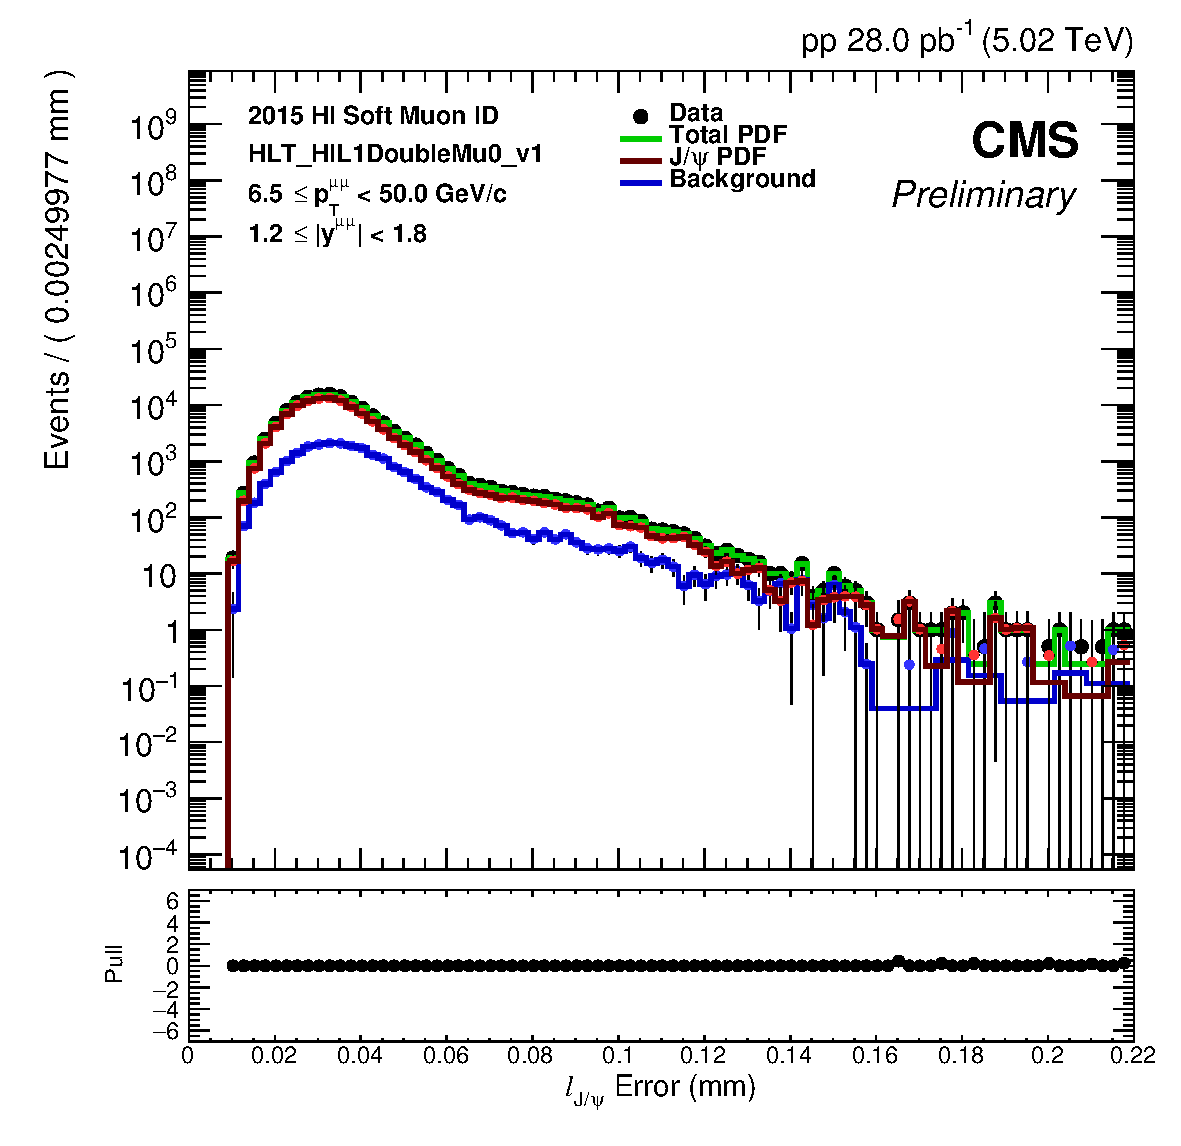
\includegraphics[width=0.45\textwidth]{Figures/Charmonia/Analysis/JpsiSignalExtraction/ctauError/PLOT_CTAUERR_DATA_PP_Jpsi_Bkg_pt65500_rap1218_cent0200.pdf}
 \caption{Distributions of the \sigmactau for signal (red line), background (blue line) and all (green line) dimuons, extracted from \RunPbPb (left) and \Runpp (right) data. The dashed lines represents the \sigmactau range used to extract the template histograms. The bottom panel shows the ratio between the data and the total template histogram extracted using the sPlot technique.}
 \label{fig:errDistr}
\end{figure}

\paragraph{Parametrisation of the \ctau resolution.} The \ctau resolution is parametrised in data from the negative tail of the \ctau signal distribution, which is due to resolution. Since both signal and background dimuons can have negative \ctau values, the contribution from each source is separated using the \sPlot technique, as was done for the \sigmactau distribution in the previous part. The resulting $\ctau < 0$ distribution, derived from the \sPlot signal-like dataset, is then fitted with a weighed sum of three Gaussian functions, defined as:

\begin{equation}
 \label{eq:CtauRes}
 \begin{aligned}
  R\left(\ctau | \sigmactau\right) &=  \frac{f^{r}_{1}}{s^{r}_{1}\sigmactau\sqrt{2\pi}} \exp\left[\frac{1}{2}\left(\frac{\ctau}{s^{r}_{1}\sigmactau}\right)^{2}\right] \\ &+ \left(1- f^{r}_{1}\right) \left[\frac{f^{r}_{2}}{s^{r}_{2}\sigmactau\sqrt{2\pi}} \exp\left[\frac{1}{2}\left(\frac{\ctau}{s^{r}_{2}\sigmactau}\right)^{2}\right] + \frac{\left(1-f^{r}_{2}\right)}{s^{r}_{3}\sigmactau\sqrt{2\pi}} \exp\left[\frac{1}{2}\left(\frac{\ctau}{s^{r}_{3}\sigmactau}\right)^{2}\right]\right]
 \end{aligned}
\end{equation}

where $s^{r}$ are scale factors that account for deviations from the measured \ctau uncertainties, and $f^{r}$ are the weights of the Gaussian components. The $s^{r}$ and $f^{r}$ parameters are left free in the fits to the data. The Gaussian mean values have been checked to be consistent with zero, and are fixed to zero in the fits. The scale factors $s^{r}_{i}$ are constrained such that $s^{r}_{3} \geq s^{r}_{2} \geq s^{r}_{1}$.

Two examples of \ctau resolution fits for \Runpp and \RunPbPb data are given in \fig{fig:ctaures_data} plotted as a function of $\ctau / \sigmactau$.

\begin{figure}[htb!]
 \centering
 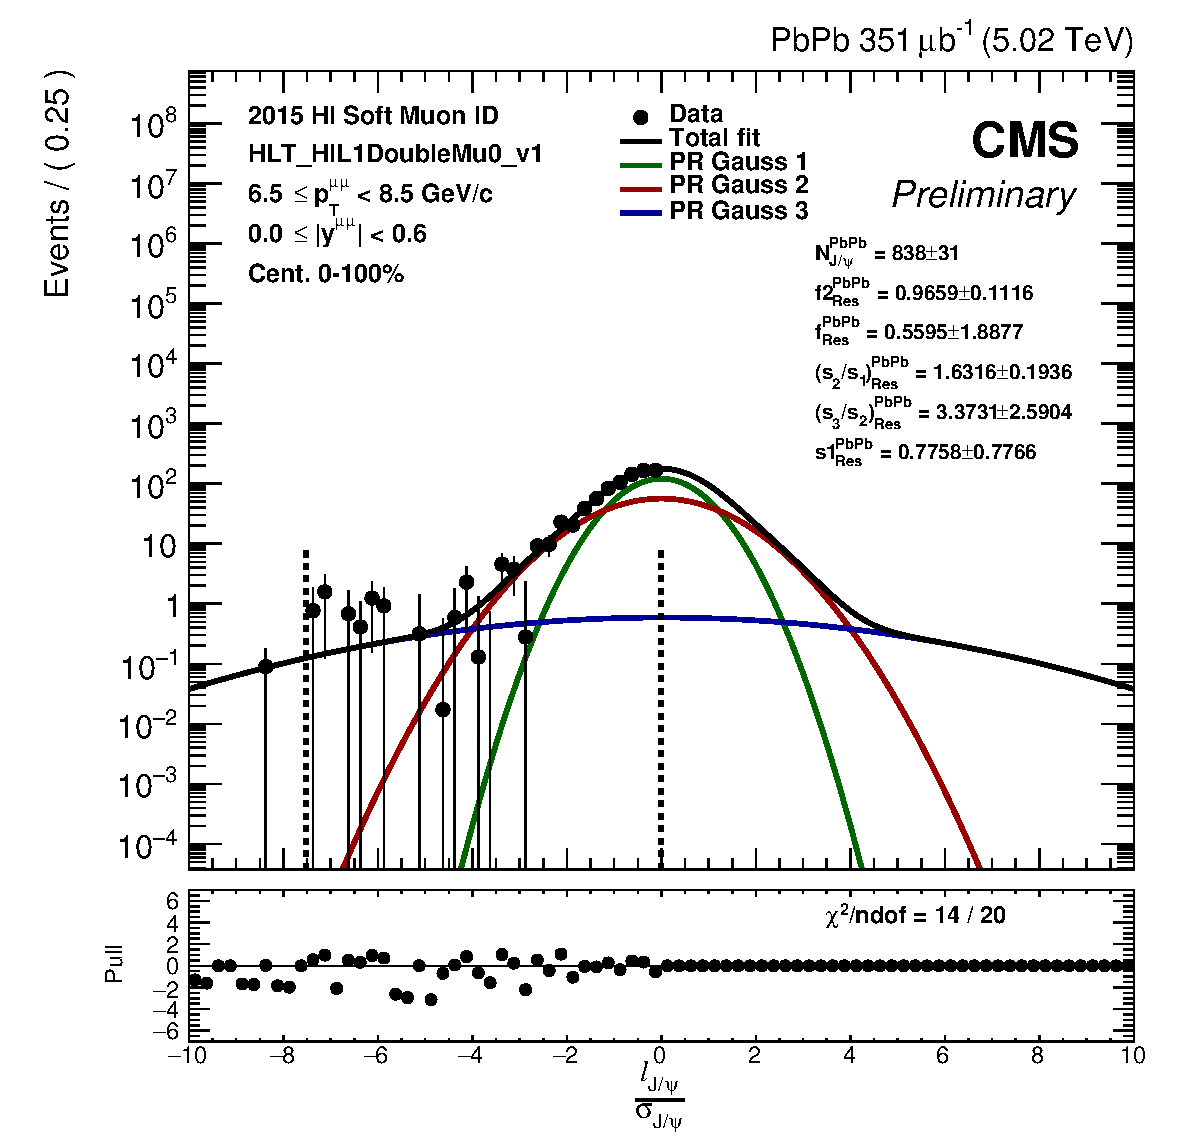
\includegraphics[width=0.45\textwidth]{Figures/Charmonia/Analysis/JpsiSignalExtraction/ctauRes/PLOT_CTAURES_DATA_PbPb_CtauRes_TripleGaussianResolution_pt6585_rap06_cent0200.pdf}
 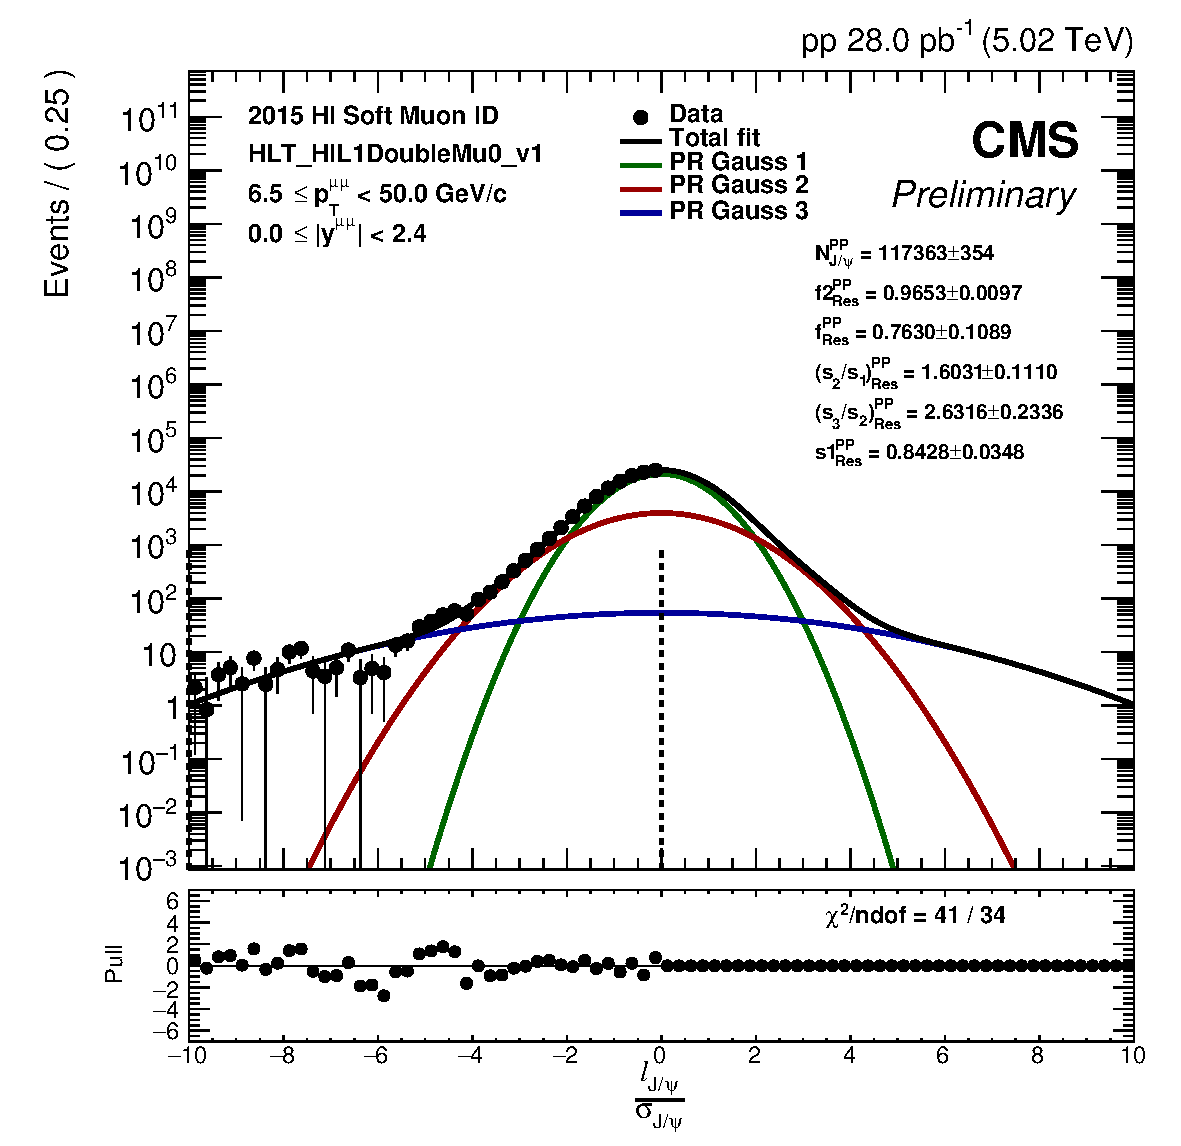
\includegraphics[width=0.45\textwidth]{Figures/Charmonia/Analysis/JpsiSignalExtraction/ctauRes/PLOT_CTAURES_DATA_PP_CtauRes_TripleGaussianResolution_pt65500_rap024_cent0200.pdf}
 \caption{Results of the \ctau resolution fits for signal dimuons in data. The results are presented as a function of $\ctau / \sigmactau$ and the dashed lines represent the fitted range.}
 \label{fig:ctaures_data}
\end{figure}

\subsubsection{Pseudoproper-decay length parametrisation}\label{sec:Charmonia_Analysis_JPsiYieldExtraction_CtauPar}

The \ctau distribution of \JPsiToMuMu events is separated in two components: prompt and nonprompt \JPsi mesons. In the case of background dimuons, the description of the \ctau distribution is also separated in a prompt and nonprompt component. On the one hand, the prompt background component represents \mumu pairs from background events whose dimuon vertex is consistent with the primary collision vertex, such as low mass Drell-Yan events. On the other hand, the nonprompt background component are made of uncorrelated muons faking  a displaced vertex.

\paragraph{Parametrisation of the \ctau true lineshape of \JPsi mesons.} The \ctau true lineshape of prompt \JPsi mesons is described with a Dirac delta function ($\delta\left(\ctau\right)$) and the one for  nonprompt \JPsi mesons is modelled with an exponential function. The signal \ctau true functional form is then given by:

\begin{equation}
 D_{\JPsi}\left(\ctau\right) = \bJPsi \cdot \exp{\left( -\abs{\lambda_{\B}} \cdot \ctau \right)} + \left(1 - \bJPsi\right) \cdot \delta\left(\ctau\right)
 \label{eq:CtauJPsi}
\end{equation}

where \bJPsi is the fraction of nonprompt \JPsi mesons and $\lambda_{\B}$ represents the average decay length of b hadrons. The $\lambda_{\B}$ parameter is initialised, when performing the 2D fits on data, to the value obtained by fitting the generated \ctau distribution of the nonprompt \JPsi simulation.

Examples of fits to the generated \ctau distribution of nonprompt \JPsi simulations are shown in \fig{fig:Jpsi_pbpb_2dfits_NPTrue} for \RunPbPb and \Runpp data (the $\lambda_{\B}$ parameter is labelled in the plots as $\lambda_{\text{DSS}}$~\footnote{The initial DSS stands for Decays on Single Side}).

\begin{figure}[htb!]
 \centering
 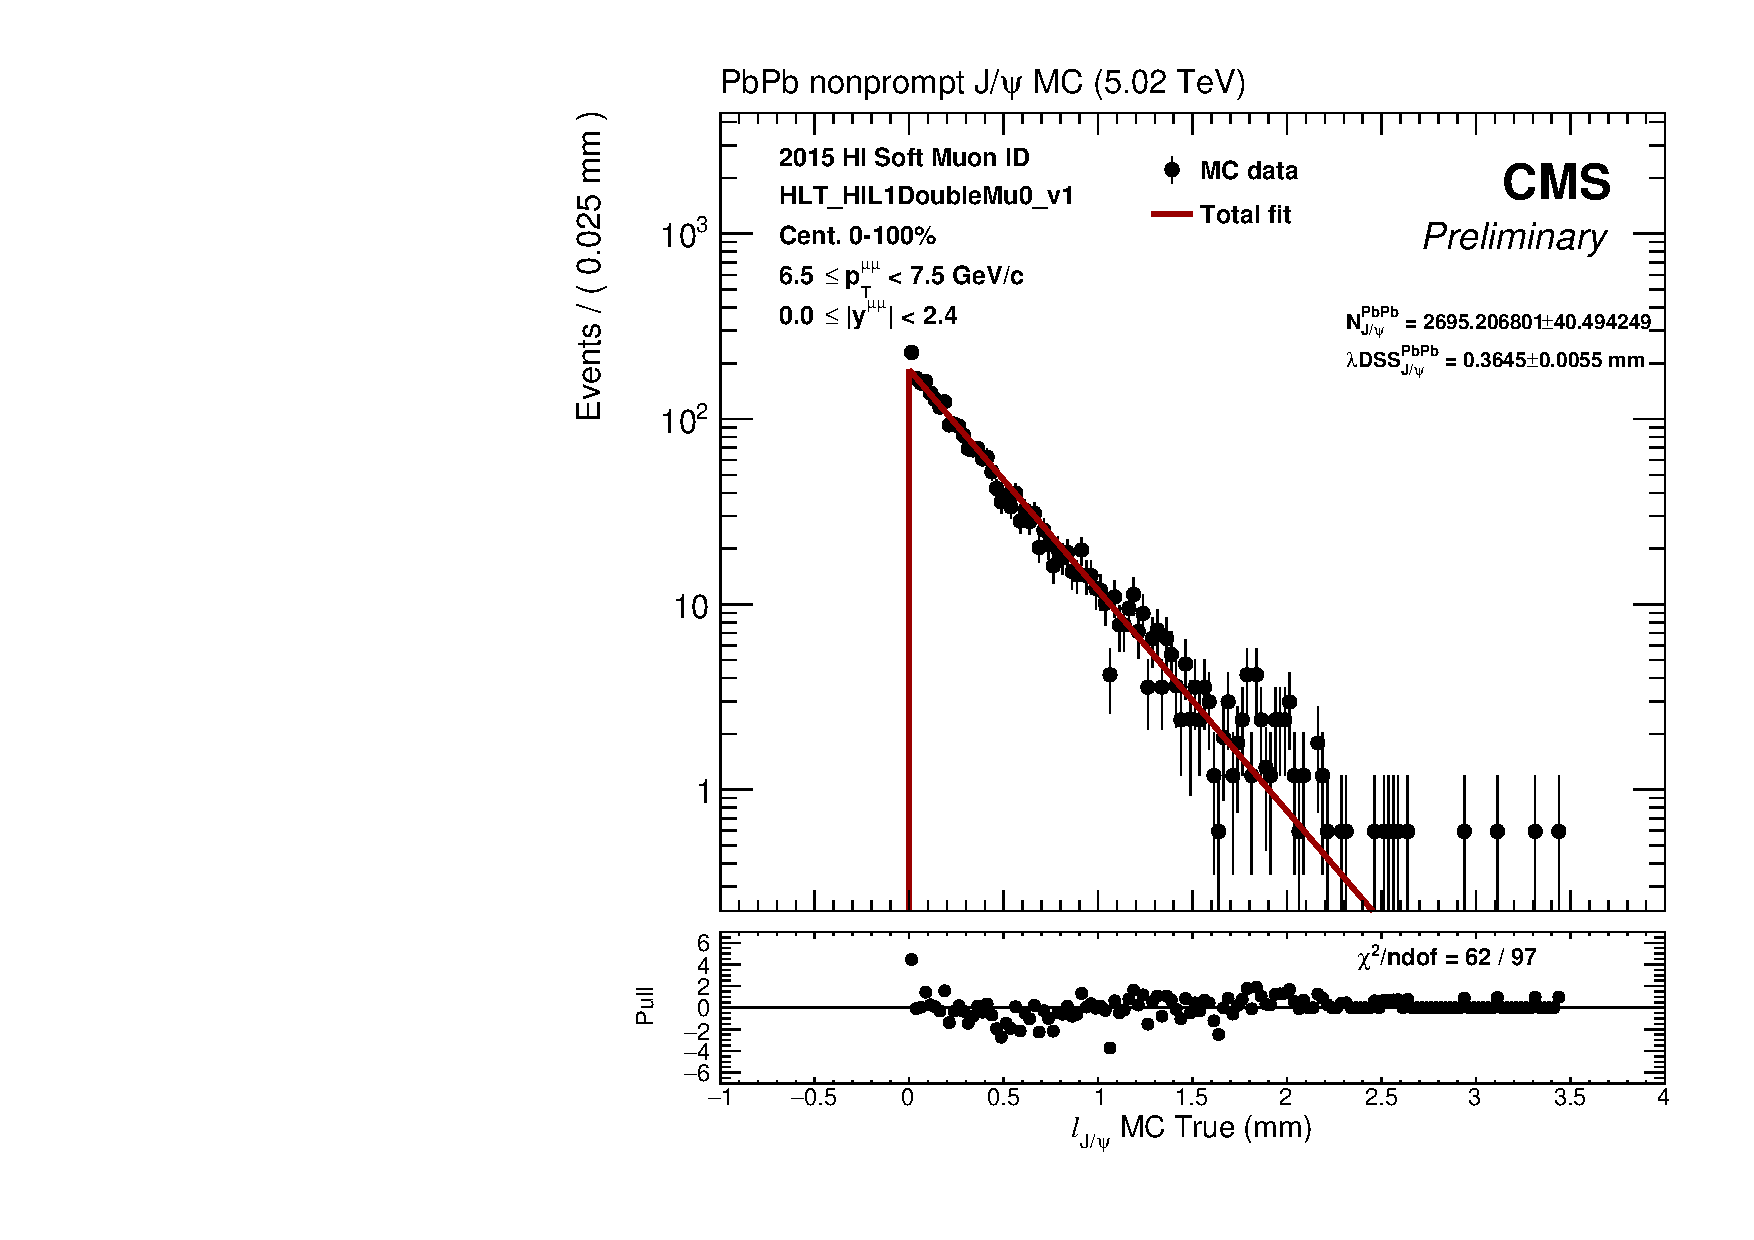
\includegraphics[width=0.45\textwidth]{Figures/Charmonia/Analysis/JpsiSignalExtraction/ctauTrue/PLOT_CTAUTRUE_MCJPSINOPR_PbPb_CtauTrue_SingleSidedDecay_NoBkg_pt6575_rap024_cent0200.pdf}
 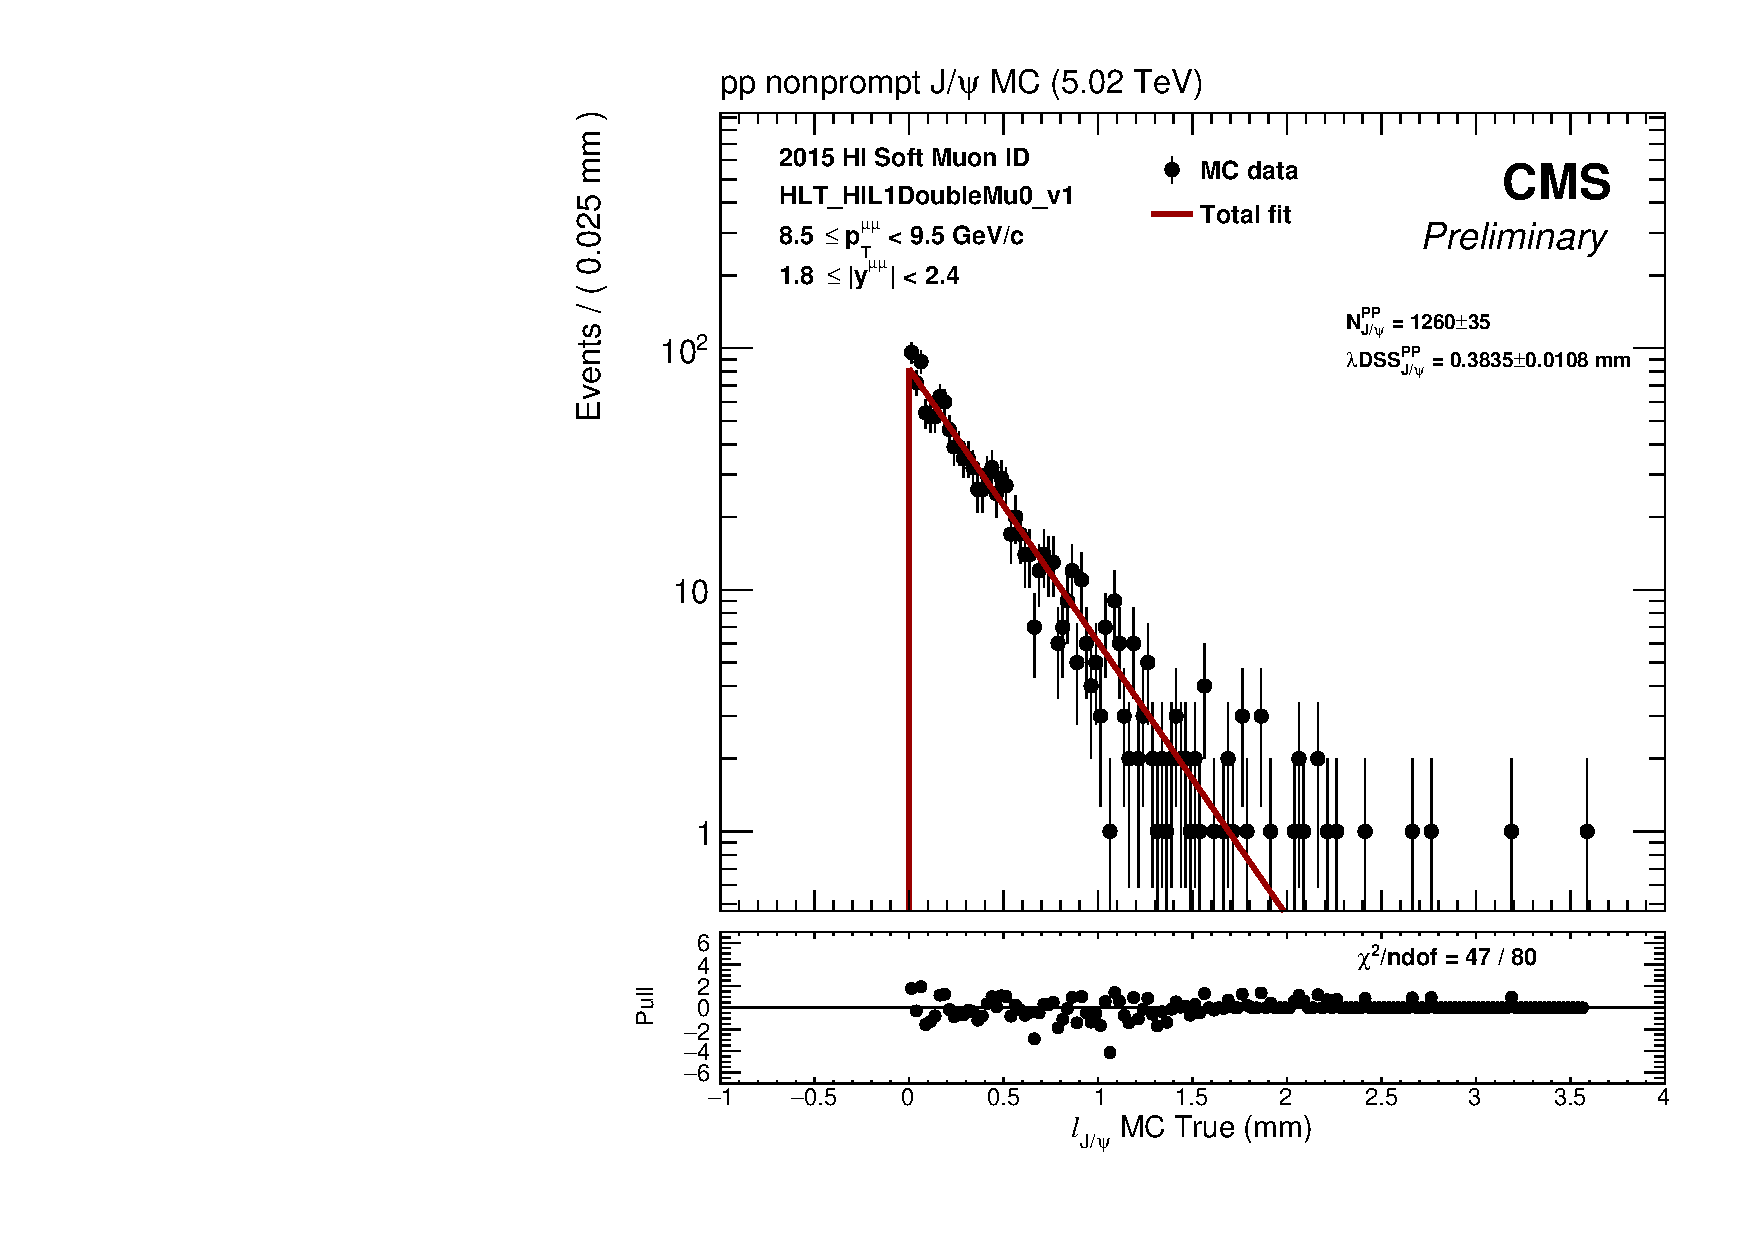
\includegraphics[width=0.45\textwidth]{Figures/Charmonia/Analysis/JpsiSignalExtraction/ctauTrue/PLOT_CTAUTRUE_MCJPSINOPR_PP_CtauTrue_SingleSidedDecay_NoBkg_pt8595_rap1824_cent0200.pdf}
 \caption{Fits to the \ctau distribution of generated nonprompt \JPsiToMuMu events in \RunPbPb (left) and \Runpp (right) simulations. The fitted value for $\lambda_{\B} = \lambda_{\text{DSS}}$ is shown.}
 \label{fig:Jpsi_pbpb_2dfits_NPTrue}
\end{figure}

\paragraph{Parametrisation of the background \ctau true lineshape.} The nonprompt component of the background \ctau true lineshape is described with a weighed sum of three exponential functions, while the prompt component is described with a Dirac delta function. The full background \ctau true model is defined as:

\begin{equation}
 \begin{aligned}
  D_{\bkg}\left(\ctau\right) &= b_{\bkg} \cdot \left\{ f_{\text{DL}} \left[ f_{\text{SS}} \cdot \exp{\left(-\abs{\lambda_{\text{SS}}} \ctau \right)} + \left(1 -  f_{\text{SS}}\right) \cdot \exp{\left(\abs{\lambda_{\text{F}}} \cdot \ctau\right)} \right] \right. \\
 \left. \right. &+ \left. \left(1 - f_{\text{DL}}\right) \cdot \exp{\left( -\abs{\lambda_{\text{DS}}} \abs{\ctau} \right) } \right\} \\
  &+ \left(1- b_{\bkg}\right) \cdot \delta\left(\ctau\right)
 \end{aligned}
 \label{eq:CtauBkg}
\end{equation}

where $b_{\bkg}$ is the fraction of nonprompt background dimuons, $f_{\text{DL}}$ and $f_{\text{SS}}$ are the weights of the exponential functions, and $\lambda_{\text{SS}}$, $\lambda_{\text{F}}$ and $\lambda_{\text{DS}}$ are the exponential parameters associated to the single sided ($\ctau > 0$), flipped ($\ctau < 0$) and double sided (symmetric \ctau) exponential decay models, respectively.

The \ctau true lineshape of the background is parametrised in data by fitting the \ctau distribution of the background-like data sample derived with the \sPlot technique. The model used to fit the data is given by:

\begin{equation}
 F_{\bkg}\left(\ctau\right) = \nbkg \cdot D_{\bkg}\left(\ctau\right) \otimes R_{\bkg}\left(\ctau\right)
\end{equation}

where the \ctau resolution parameters have been fixed to data as detailed in \sect{sec:Charmonia_Analysis_JPsiYieldExtraction_CtauResPar}, and only the \nbkg and the $D_{\bkg}$ parameters ($\lambda$, $f$ and $b_{\bkg}$) are left free. Examples of fits to the \ctau distribution of background dimuons are shown in \fig{fig:ctauBkg} for \Runpp and \RunPbPb data.

\begin{figure}[htb!]
 \centering
 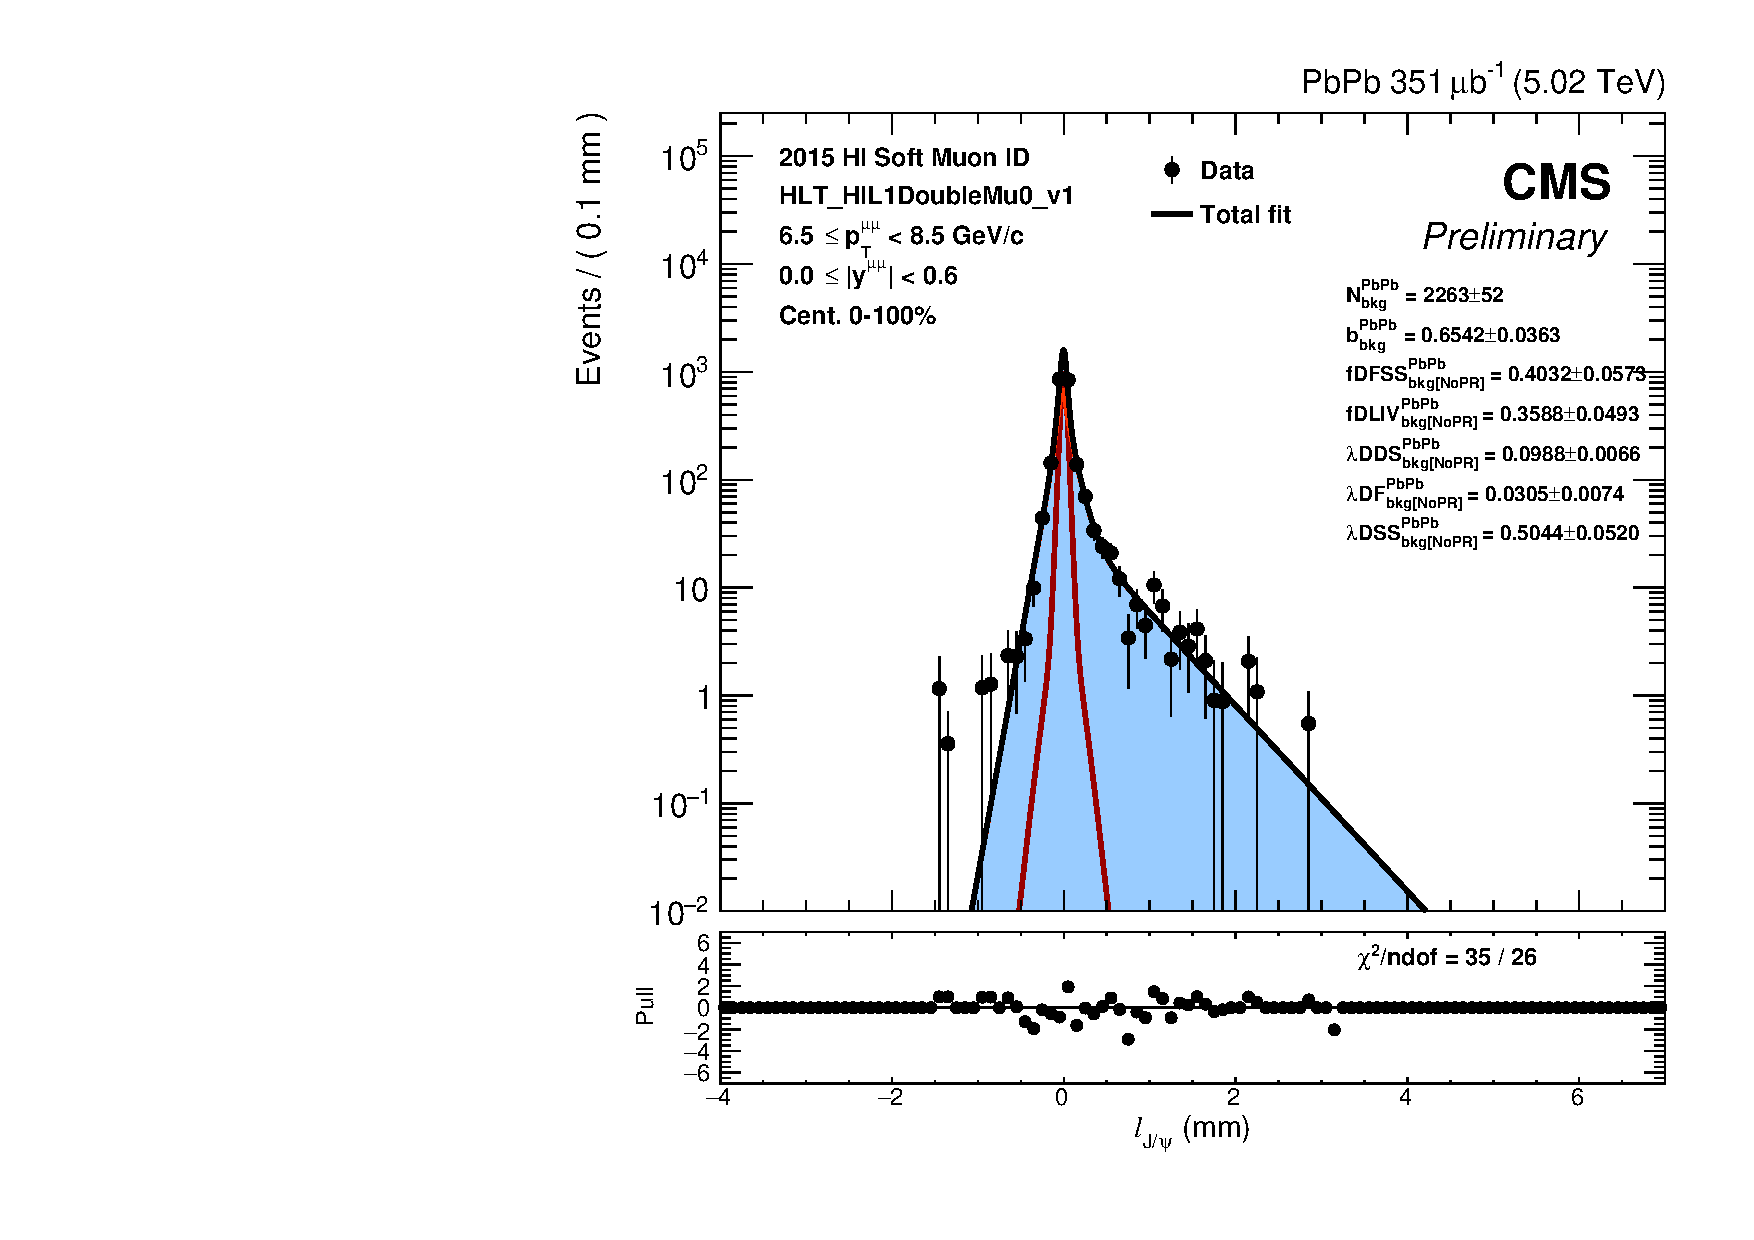
\includegraphics[width=0.45\textwidth]{Figures/Charmonia/Analysis/JpsiSignalExtraction/ctauBkg/PLOT_CTAU_DATA_PbPb_BkgNoPR_TripleDecay_CtauRes_TripleGaussianResolution_pt6585_rap06_cent0200.pdf}
 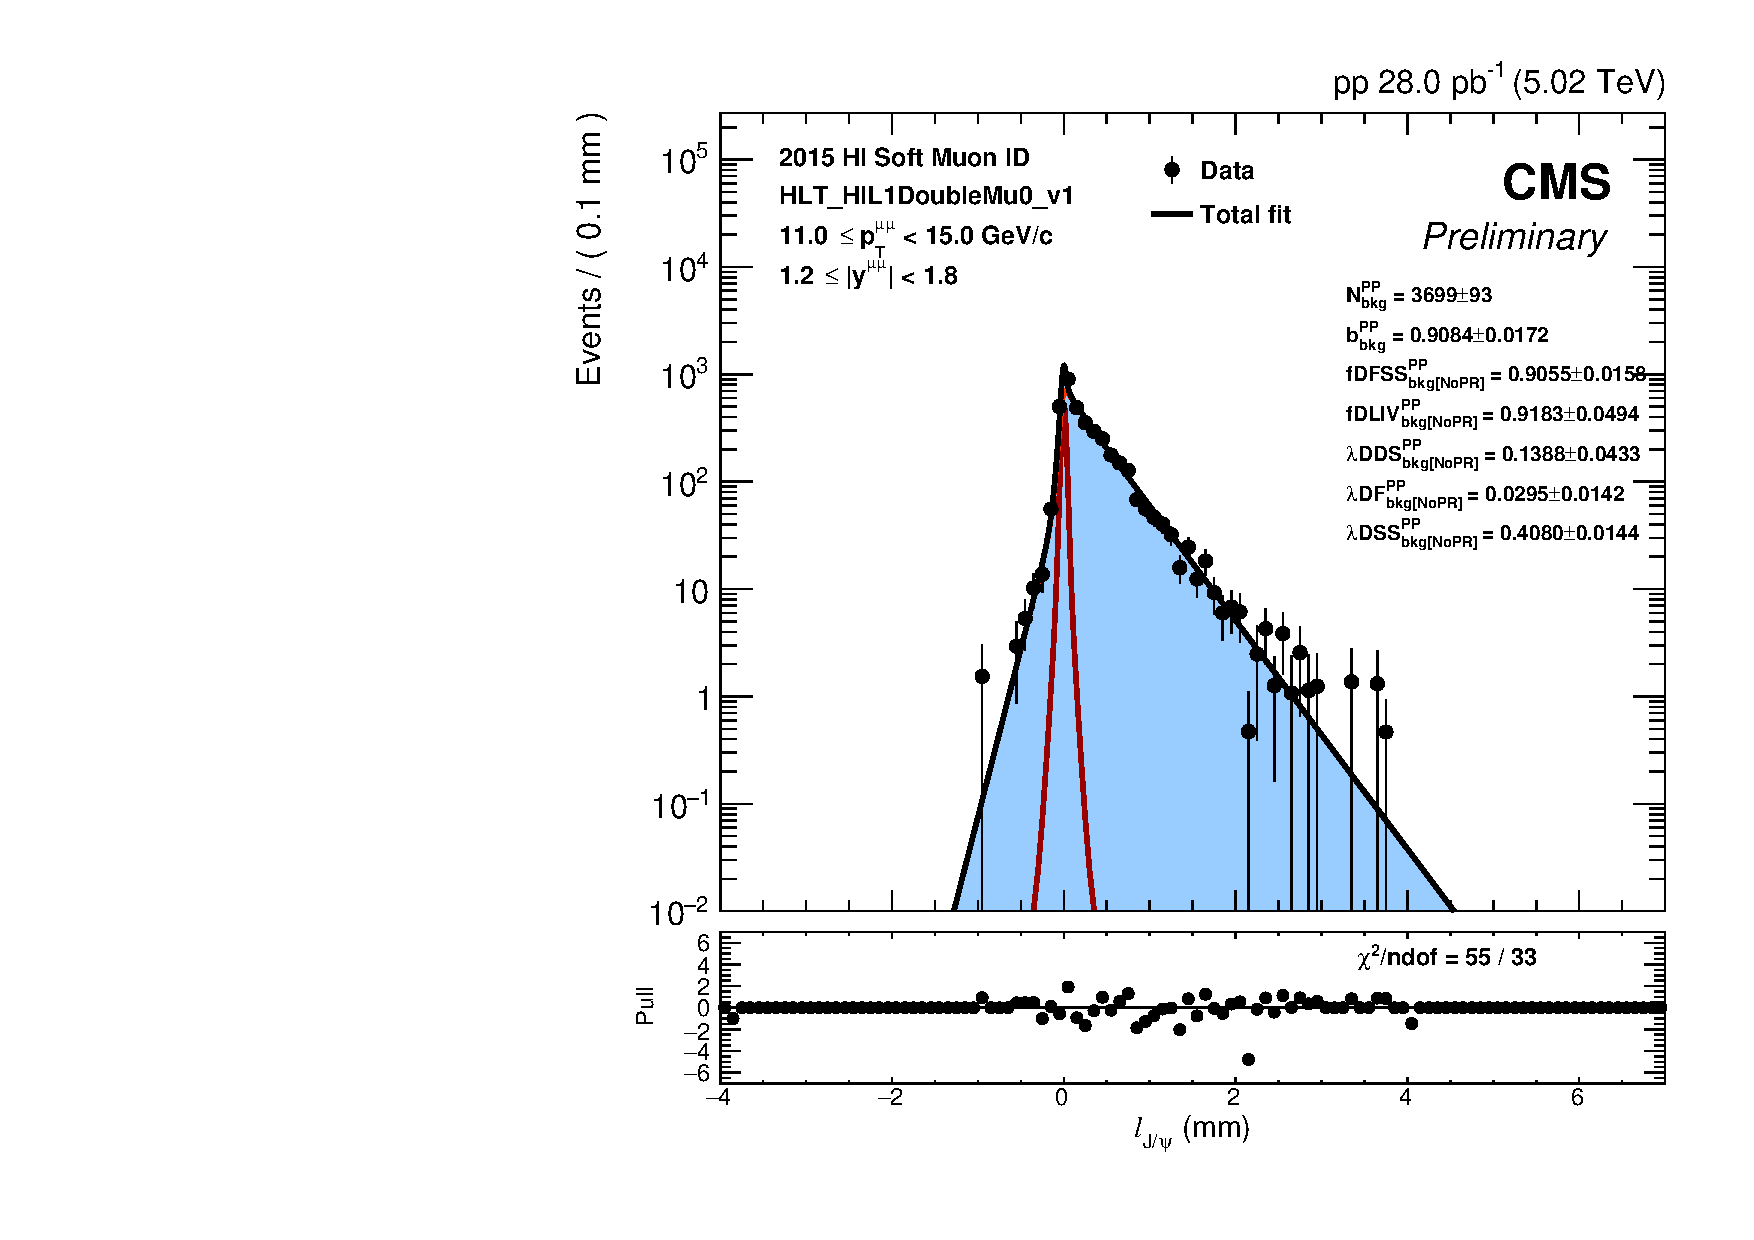
\includegraphics[width=0.45\textwidth]{Figures/Charmonia/Analysis/JpsiSignalExtraction/ctauBkg/PLOT_CTAU_DATA_PP_BkgNoPR_TripleDecay_CtauRes_TripleGaussianResolution_pt110150_rap1218_cent0200.pdf}
 \caption{Fits to the \ctau distribution of background events in \RunPbPb (left) and \Runpp (right) collision data.} 
 \label{fig:ctauBkg}
\end{figure}

\subsubsection{Two-dimensional fit to the \mMuMu and \ctau distributions}\label{sec:2Dfits}

The 2D fits to the \mMuMu and \ctau distributions represents the last step in the procedure to extract the \JPsi-meson yields. The parameters used in the 2D fit model are fixed as explained in the previous sections, except for the average decay length of b hadrons $\lambda_{\B}$, the fraction of nonprompt \JPsi-mesons \bJPsi, the inclusive \JPsi-meson yield \nJPsi, and the background yield \nbkg. \fig{fig:2DFits_proj} shows an example of 2D fit extracted from \RunPbPb collision data.

\subsubsection{Prompt and nonprompt \texorpdfstring{\JPsi}{J/psi} meson yields}\label{sec:JPsiYields}

Finally, the yields of the prompt ($N^{\text{P}}_{\JPsi}$) and nonprompt ($N^{\text{NP}}_{\JPsi}$) \JPsi mesons are simply derived from the number of inclusive \JPsi mesons \nJPsi and the fraction of nonprompt \JPsi mesons \bJPsi, according to:

\begin{equation}
 \begin{aligned}
  N^{\text{P}}_{\JPsi} &= (1-\bJPsi) \cdot \nJPsi \\
  N^{\text{NP}}_{\JPsi} &= \bJPsi \cdot \nJPsi
 \end{aligned}
 \label{PnNPJpsi}
\end{equation}

and the corresponding statistical uncertainty are computed using error propagation and taking into account the correlation between \bJPsi and \nJPsi, determined from the 2D fits.

% END OF SUBSECTION